\chapter{Конструкторская часть}

В данном разделе будут рассмотрены алгоритмы 
конвейерной и последовательной обработок, а также 
алгоритм нахождения обратной матрицы методом Жордана-Гаусса, стандартный 
алгоритм умножения матриц, алгоритм Винограда для умножения матриц.


\section{Разработка алгоритмов}

На рисунке \ref{fig:posled} представлена схема линейного алгоритма обработки заявок.
На рисунке \ref{fig:pipOsn} представлена схема главного потока,
запускающего потоки обработчиков конвейера, схемы алгоритмов которых представлены на
рисунках \ref{fig:pip1}-\ref{fig:pip3}.

На рисунках \ref{fig:gauss1} --- \ref{fig:gauss2} представлена схема алгоритма нахождения обратной матрицы,
на рисункe \ref{fig:standartAlg} --- схема алгоритма умножения матриц стандартным методом, на рисунках 
\ref{fig:WinogradOptA}---\ref{fig:WinogradOptD} --- схема умножения матриц алгоритмом Винограда.

\begin{figure}[h]
    \centering
    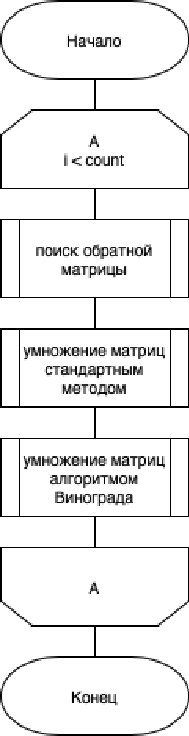
\includegraphics[width=0.3\linewidth]{img/posled.pdf}
    \caption{Схема алгоритма линейной обработки заявок}
    \label{fig:posled}
\end{figure}

\begin{figure}[h]
    \centering
    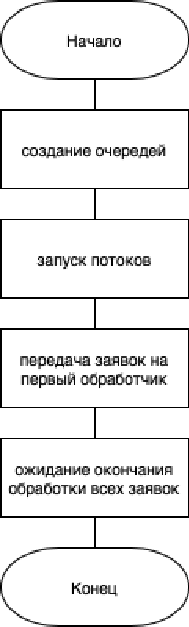
\includegraphics[width=0.3\linewidth]{img/pipOsn.pdf}
    \caption{Схема главного потока конвейерной обработки заявок}
    \label{fig:pipOsn}
\end{figure}

\begin{figure}[h]
    \centering
    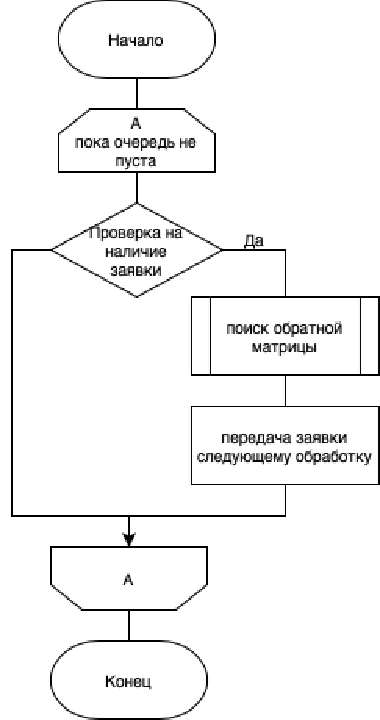
\includegraphics[width=0.6\linewidth]{img/pip1.pdf}
    \caption{Схема потока первого этапа обработки}
    \label{fig:pip1}
\end{figure}

\begin{figure}[h]
    \centering
    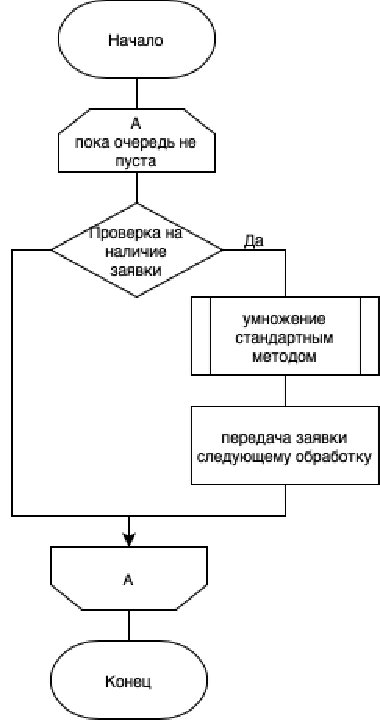
\includegraphics[width=0.6\linewidth]{img/pip2.pdf}
    \caption{Схема потока второго этапа обработки}
    \label{fig:pip2}
\end{figure}

\begin{figure}[h]
    \centering
    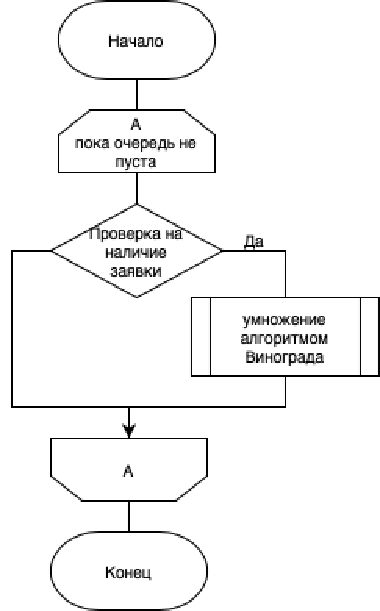
\includegraphics[width=0.6\linewidth]{img/pip3.pdf}
    \caption{Схема потока третьего этапа обработки}
    \label{fig:pip3}
\end{figure}

\begin{figure}[h]
    \centering
    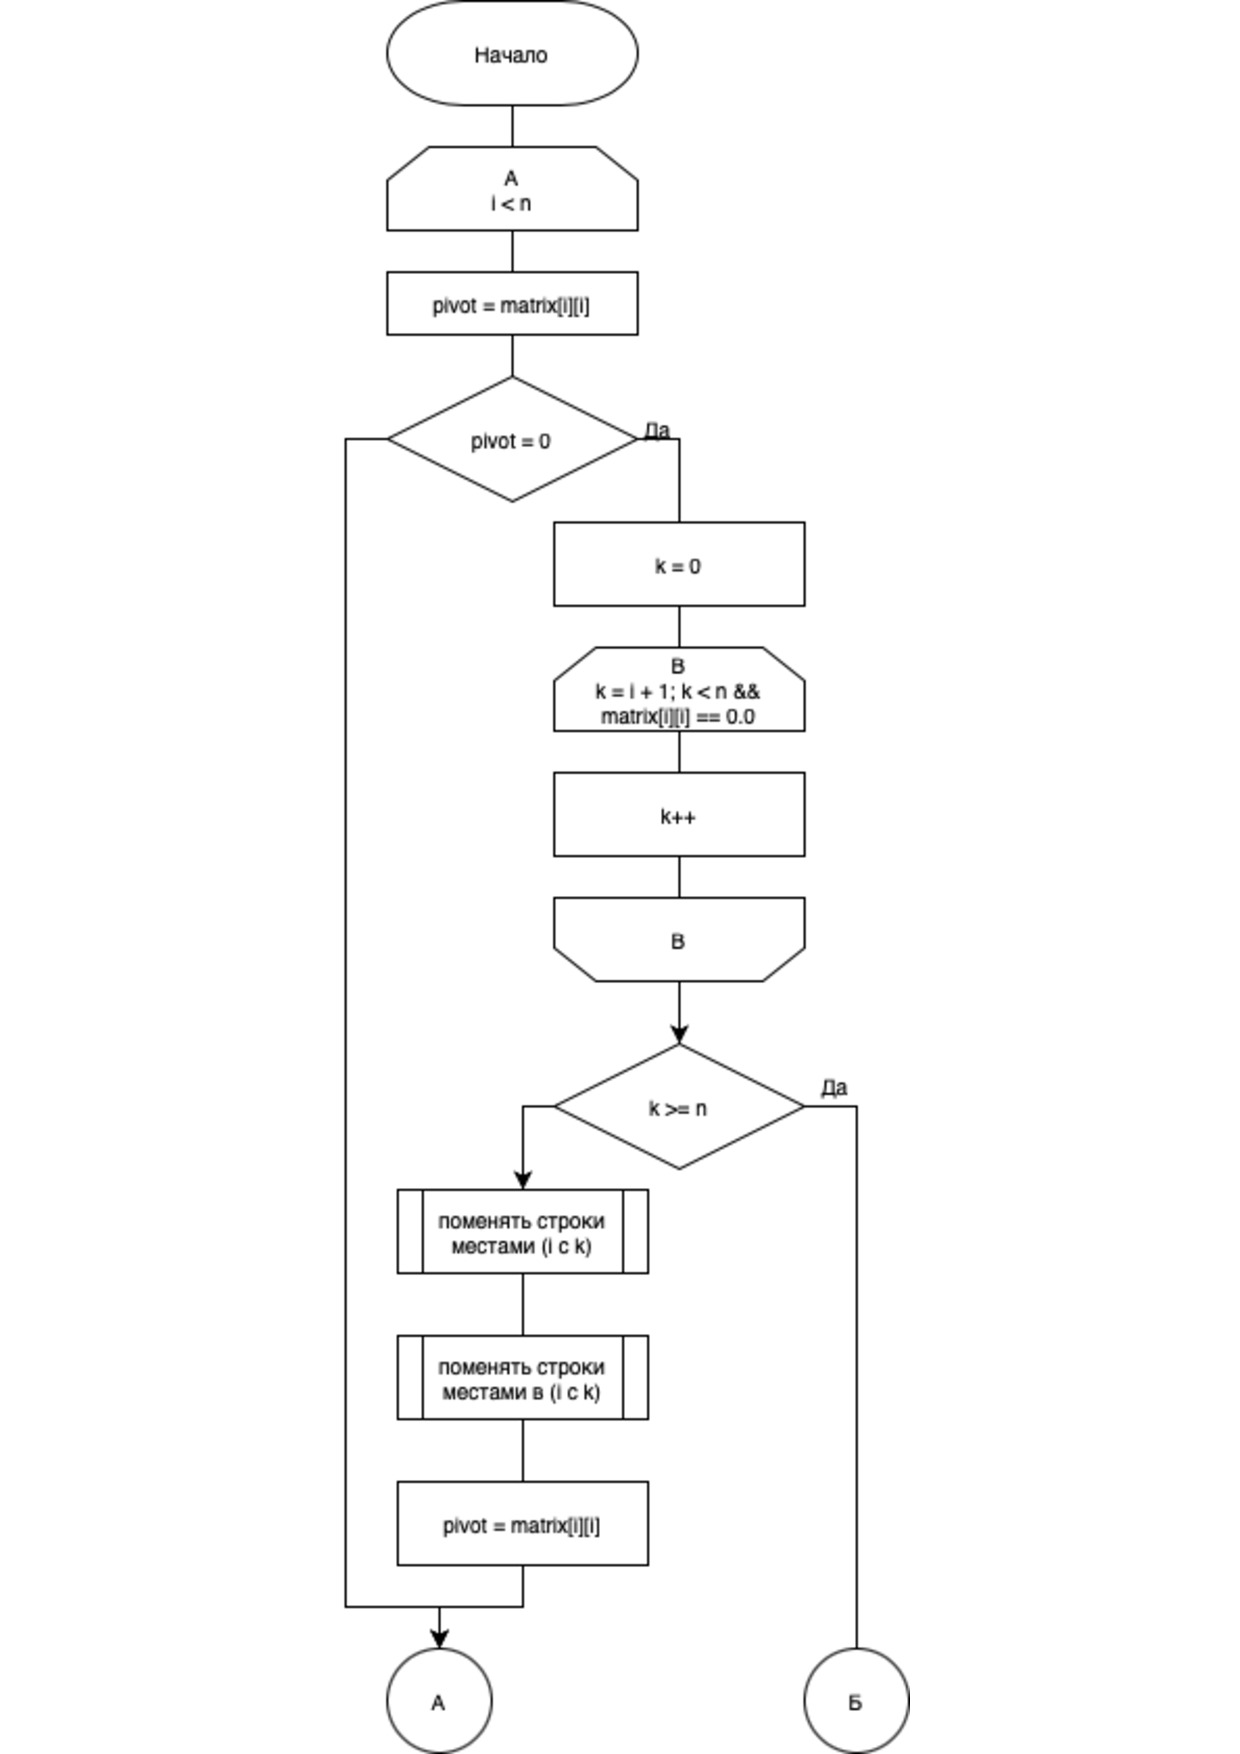
\includegraphics[width=1\linewidth]{img/gauss1.pdf}
    \caption{Схема алгоритма поиска обратной матрицы методом Жордана-Гаусса. Часть 1}
    \label{fig:gauss1}
\end{figure}

\begin{figure}[h]
    \centering
    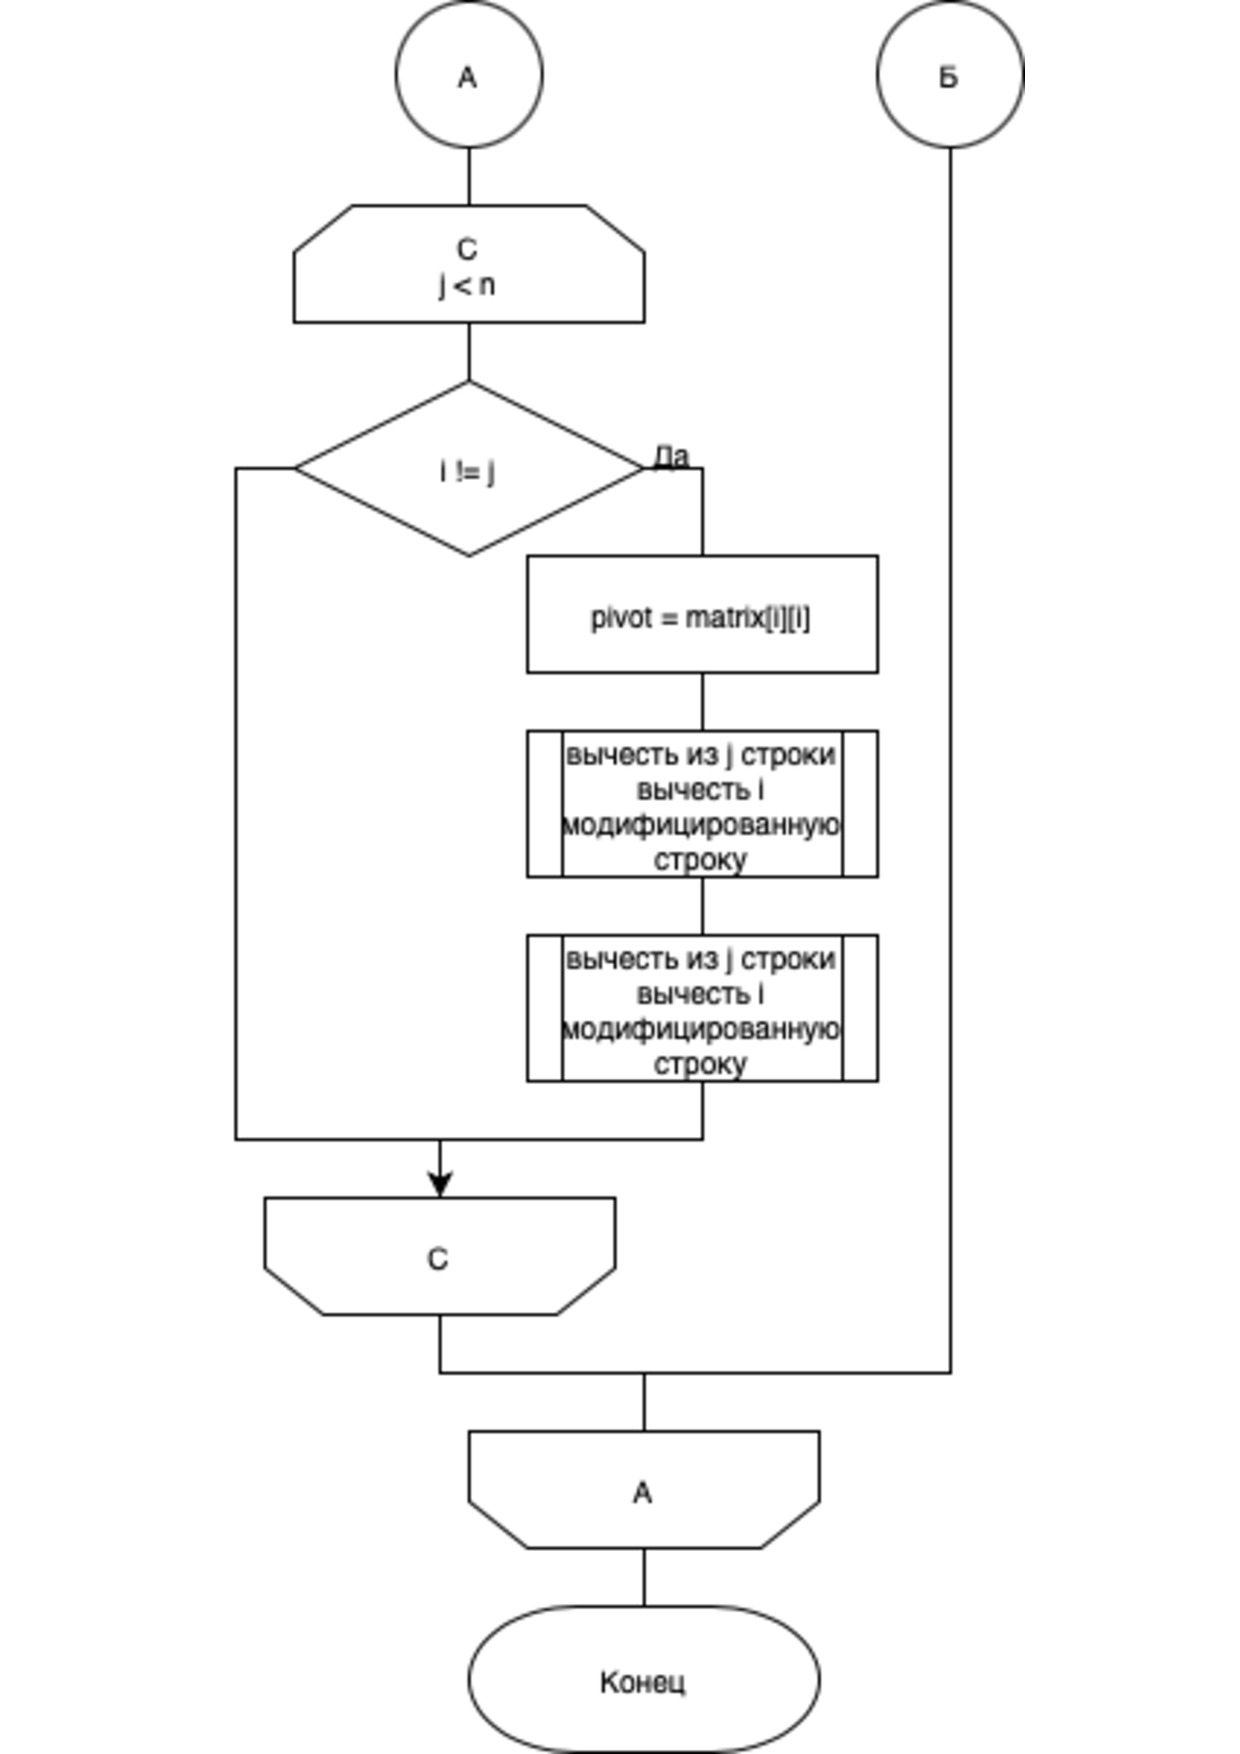
\includegraphics[width=0.9\linewidth]{img/gauss2.pdf}
    \caption{Схема алгоритма поиска обратной матрицы методом Жордана-Гаусса. Часть 2}
    \label{fig:gauss2}
\end{figure}

\begin{figure}[h]
    \centering
    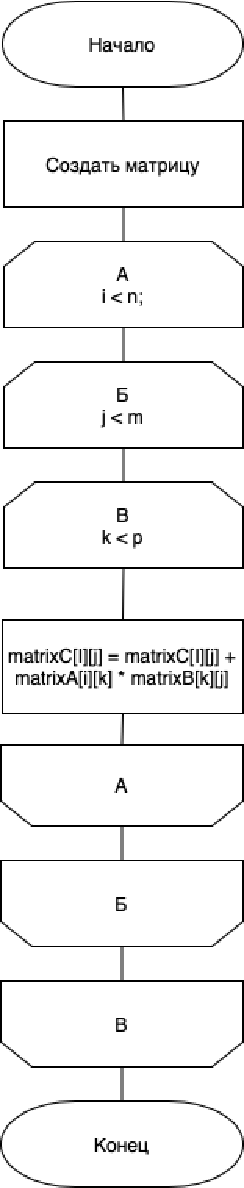
\includegraphics[width=0.3\linewidth]{img/standartAlg.pdf}
    \caption{Схема алгоритма умножения матриц стандартным методом}
    \label{fig:standartAlg}
\end{figure}

\begin{figure}[h]
    \centering
    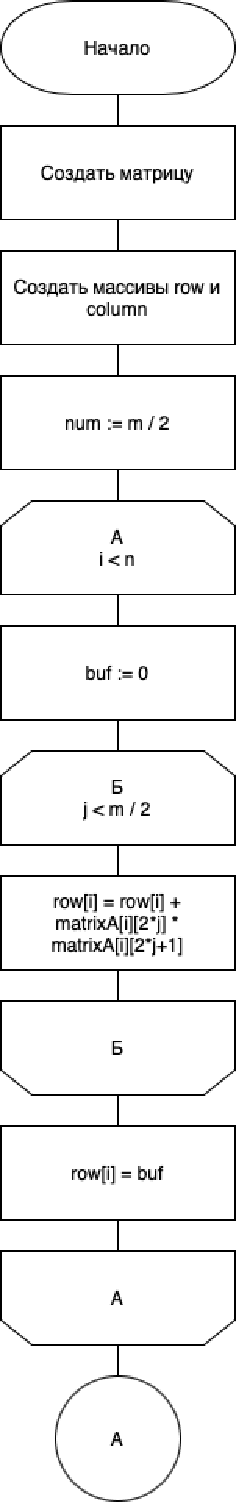
\includegraphics[width=0.22\linewidth]{img/WinogradOptA.pdf}
    \caption{Схема алгоритма Винограда. Часть 1}
    \label{fig:WinogradOptA}
\end{figure}

\begin{figure}[h]
    \centering
    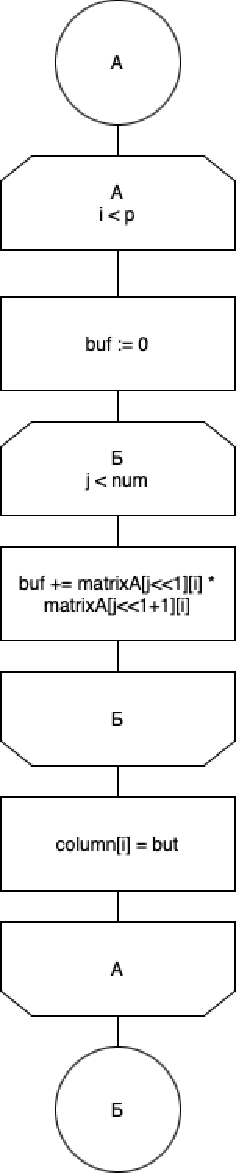
\includegraphics[width=0.28\linewidth]{img/WinogradOptB.pdf}
    \caption{Схема алгоритма Винограда. Часть 2}
    \label{fig:WinogradOptB}
\end{figure}

\begin{figure}[h]
    \centering
    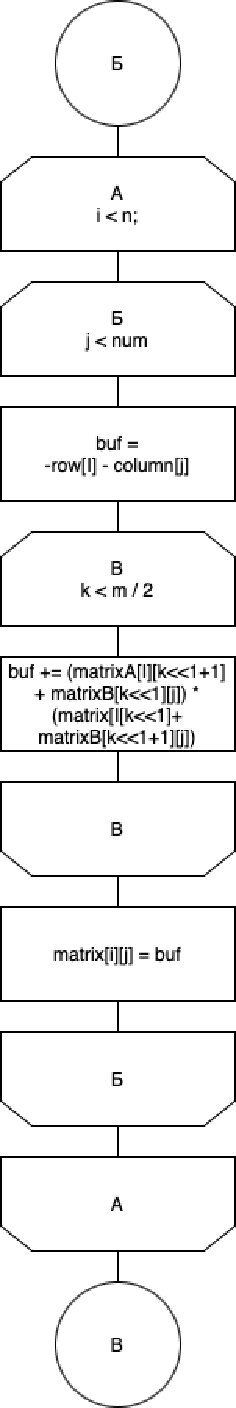
\includegraphics[width=0.24\linewidth]{img/WinogradOptC.pdf}
    \caption{Схема алгоритма Винограда. Часть 3}
    \label{fig:WinogradOptC}
\end{figure}

\begin{figure}[h]
    \centering
    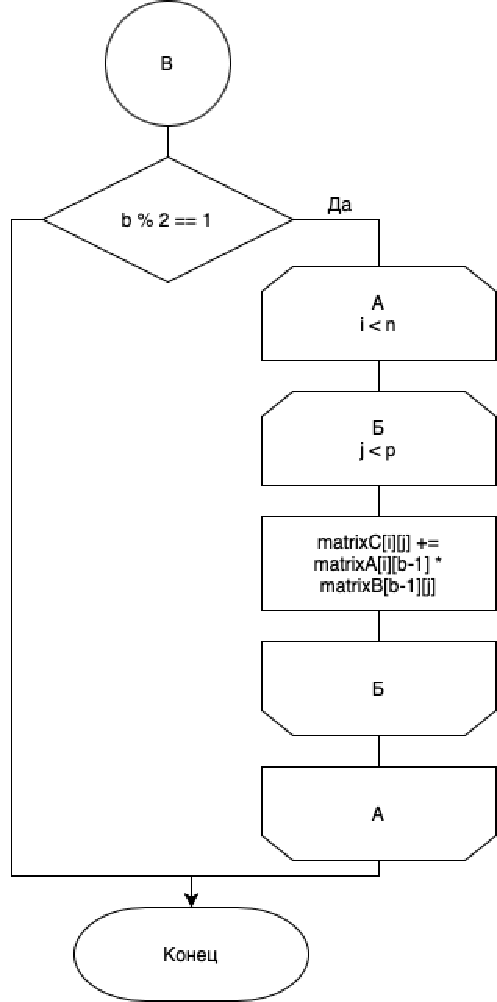
\includegraphics[width=0.55\linewidth]{img/WinogradOptD.pdf}
    \caption{Схема алгоритма Винограда. Часть 4}
    \label{fig:WinogradOptD}
\end{figure}

\clearpage
\section{Структура разрабатываемого программного обеспечения}

Для реализации разрабатываемого программного обеспечения будет использоваться
метод структурного программирования. Каждый из алгоритмов будет представлен
отдельной функцией, при необходимости будут выделены подпрограммы для каждой из
них. Также будут реализованы функции для ввода-вывода и функция, вызывающая все
подпрограммы для связности и полноценности программы.

\section{Требования к программному обеспечению}

Программа должна предоставлять следующие возможности:
\begin{itemize}[left=\parindent]
    \item ввод количества обрабатываемых заявок, размерности матриц, элементов матриц;
    \item вывод результата работы программы;
    \item замер времени работы алгоритмов;
\end{itemize}

\section*{Вывод}

В данном разделе были разработаны алгоритмы этапов обработки матриц, а также алгоритмы
линейной и конвейерной обработки заявок, была описана структура разрабатываемого программного
обеспечения.
